\documentclass[a4paper,twoside]{article}

\usepackage{epsfig}
\usepackage{subfigure}
\usepackage{calc}
\usepackage{amssymb}
\usepackage{amstext}
\usepackage{amsmath}
\usepackage{amsthm}
\usepackage{multicol}
\usepackage{pslatex}
\usepackage{apalike}
\usepackage{SciTePress}
\usepackage[small]{caption}
\usepackage{epstopdf}
\usepackage[utf8]{inputenc}
\usepackage[ngerman,english]{babel}
\usepackage{listings}

\lstdefinestyle{myCustomUseStyle}{
  stepnumber=1,
  numbersep=10pt,
  tabsize=3,
  showspaces=false,
  showstringspaces=false
}

\subfigtopskip=0pt
\subfigcapskip=0pt
\subfigbottomskip=0pt

\begin{document}

\title{\uppercase{Modellgetriebene Entwicklung einer mobilen Applikation mit JUSE4Android}}

\author{\authorname{Jano Espenhahn, Tobias Franz and Franziska Krebs}
\affiliation{Fachhochschule Brandenburg, Fachbereich Informatik und Medien}
\email{\{espenhah, franzt, krebsf\}@fh-brandenburg.de}
}

\keywords{MDA, UML, USE, OCL, Android}

\abstract{ein deutsches Abstract}{ein englisches Abstract}


\onecolumn \maketitle \normalsize \vfill

\section{\uppercase{Einleitung}}
\label{sec:introduction}
\noindent Zitat Test
\cite{SilvaMasterThesis}

\section{\uppercase{Vorstellung USE}}

UML based Specifiation Environment (USE) wird zur Spezifikation von Informationssystemen verwendet und wurde an der Universität Bremen entwickelt. Neben dem Einsatz für Fallstudien, wird USE vor allem in der Lehre an Hochschule wie z. B. MIT, Cambridge, University of Edinburgh und University of Lisbon eingesetzt.  USE basiert auf einer Teilmenge der Unified Modeling Language (UML) und der Object Constraint Language (OCL). Eine USE-Spezifikation besteht aus einer textuellen Beschreibung eines Modells, bei der Eigenschaften aus UML-Diagramm verwendet werden. Weitere Integritätsausdrücke für ein Modell können durch die OCL definiert werden. \cite{Use07} Die OCL wird im späteren Kapitel (TODO) vorgestellt. Die nachfolgende Abbildung veranschaulicht den Workflow für eine USE-Spezifikation.

\begin{figure}[!h]
	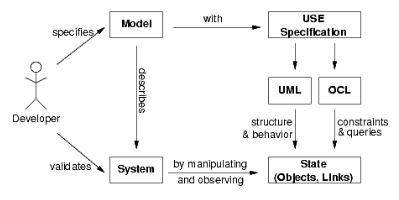
\includegraphics[scale=.7]{pics/USE_workflow.jpg}
	\captionsetup{labelformat=empty}
	\caption{Workflow einer USE-Spezifikation \cite{Data07}}
\end{figure}

Ein Entwickler spezifiziert ein USE-Modell, welches ein System beschreibt und nutzt dafür UML- und OCL-Ausdrücke. Mithilfe von USE ist es ihm möglich die bestimmten Anforderungen an sein System auf Erfüllung mit dem Modell zu validieren.

\subsection{Spezifikation}

Die textuelle Beschreibung eines Modells mit USE beginnt immer mit der Definition eines Modell-Namens. In diesem Fall ist das \textit{IceCream}. Im Anschluss folgen Klassendefinitionen mit ihren jeweiligen Attributen und Methoden. Im Beispiel hat die Klasse \textit{Station} das Attribut \textit{name} und die Operation \textit{entries} ohne Übergabeparameter. Die nachfolgenden Code-Ausschnitte verwenden lediglich UML.

\lstset{basicstyle=\tiny,style=myCustomUseStyle}
\begin{lstlisting}
model IceCream

class Station
	attributes
		name			: String
	operations
		entries()	: Set(Entry) = self.records->asSet
end
\end{lstlisting}

Klassen können untereinander in Abhängigkeit stehen. Für diese Abhängigkeiten sind Assoziationen vorgesehen. Um eine Assoziation auszudrücken, wird zuerst eine weitere Klasse \textit{Address} eingeführt.

\begin{lstlisting}
class Address
	attributes
		street	: String
		postCode	: Integer
end
\end{lstlisting}

Für das dem Artikel zugrunde liegende Beispiel kann eine Station entweder eine oder keine Adresse haben.

\begin{lstlisting}
association Station_Address between
	Station[ 1 ] 
	Address[ 0..1 ] role place
end
\end{lstlisting}

\textit{Station\_Address} ist dabei der Name der Assoziation und das Attribut \textit{place} nimmt in der Klasse \textit{Station} die Rolle für die Adresse ein. Zum gesamten USE-Modell gehören weiterhin noch die Klasse \textit{Entry} und die Assoziation \textit{Station\_Entry}.

\begin{lstlisting}
class Entry
	attributes
		date		: CalendarDate
		target		: Integer
		actual		: Integer
		variance	: Integer
	operations
		variance(): Integer = actual - target	
end

association Station_Entry between
	Station[ 1 ] 
	Entry[ * ] role records
end
\end{lstlisting}

Zur Vervollständigung des Modells gehört außerdem eine aus der Arbeit \cite{SilvaMasterThesis} entnommene Klasse \textit{CalendarDate}.

\subsection{Tool}

Um eine Spezifikation auf nicht-formale Anforderungen zu validieren, kann ein Modell mithilfe des USE-Tools animiert werden. Direkt nach dem Import eines Modells erhält man vom Tool ein Feedback über die Validität der UML- und OCL-Definitionen. Neben der Validierung bietet das Tool weitere Möglichkeiten, wie z. B. die Visualisierung eines Klassen-, Sequenz- oder Objektdiagramms.

\begin{figure}[!h]
	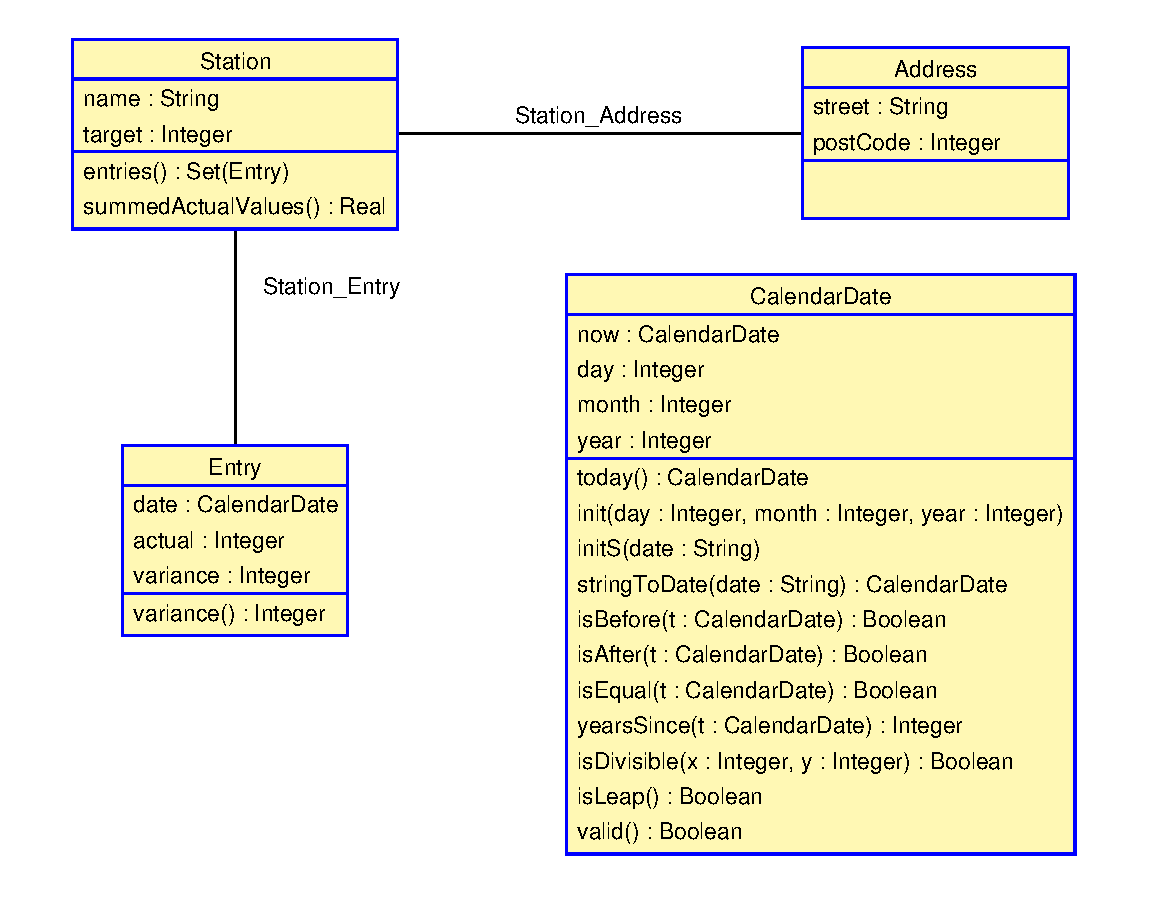
\includegraphics[scale=.45]{pics/USE_class_diagramm.pdf}
	\captionsetup{labelformat=empty}
	\caption{Klassendiagramm für das Beispiel}
\end{figure}

\section{\uppercase{Vorstellung OCL}}

\section{\uppercase{JUSE4Android}}

\vfill
\bibliographystyle{apalike}
{\small
\bibliography{bib/literature}}

\section*{\uppercase{Anhang}}

\noindent If any, the appendix should appear directly after the
references without numbering, and not on a new page. To do so please use the following command:
\textit{$\backslash$section*\{APPENDIX\}}


\vfill
\end{document}

